\subsection{Hyperbolic space}
From the visual standpoint, the hyperbolic space can be identified by the fact that the otherwise flat terrain appears "curved downward".
This may create an illusion that the terrain is wrapped around a giant sphere.
\todo{That's at least how it looks to me}
However, by exploring the hyperbolic space, we can quickly notice that it is infinite, just like the Euclidean space.
\autoref{fig:hyperbolic-space-games} shows the comparison of the depictions of hyperbolic space between our game and \textit{Hyperbolica}.
\begin{figure*}[h]
    \centering
    \begin{subfigure}[b]{0.475\textwidth}
        \centering
        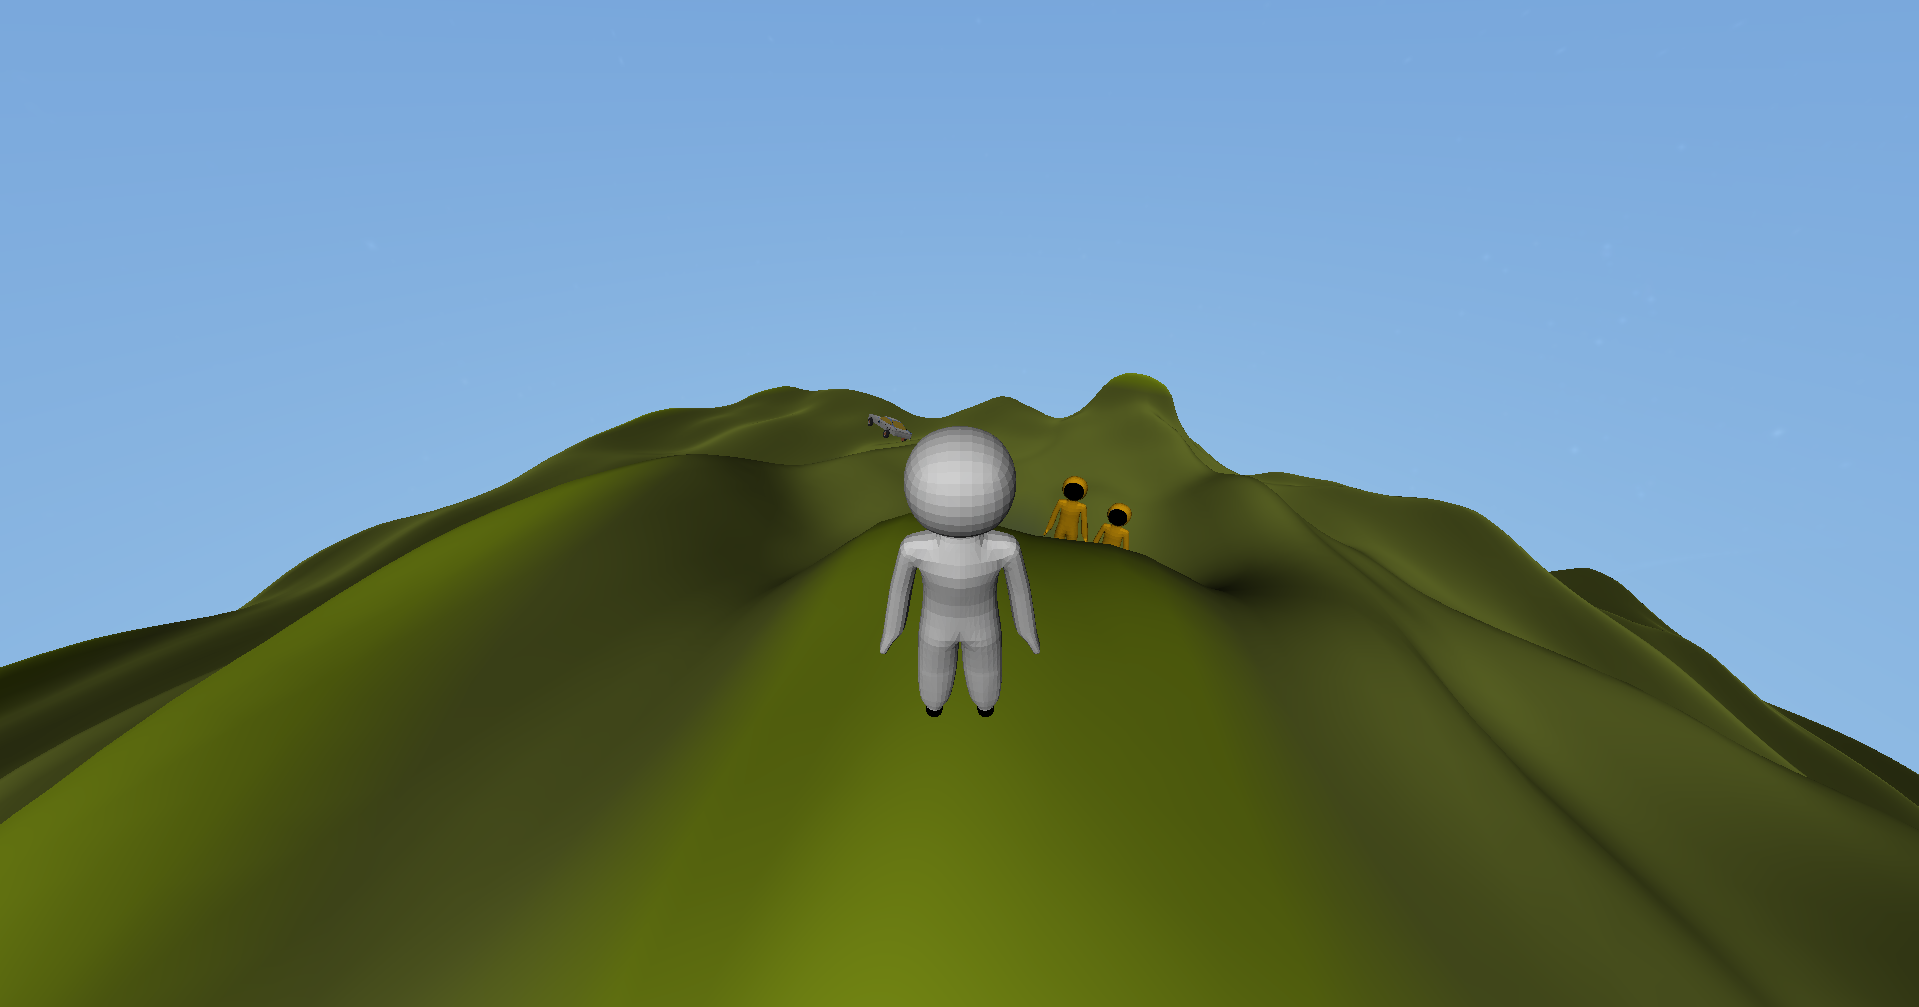
\includegraphics[width=\textwidth]{chapters/results/sections/non_euclidean/resources/hyperbolic-in-hyper.png}
        \caption[]%
        {{\small \textit{Hyper}}}
        \label{fig:hyperbolic-space-games-hyper}
    \end{subfigure}
    \hfill
    \begin{subfigure}[b]{0.475\textwidth}
        \centering
        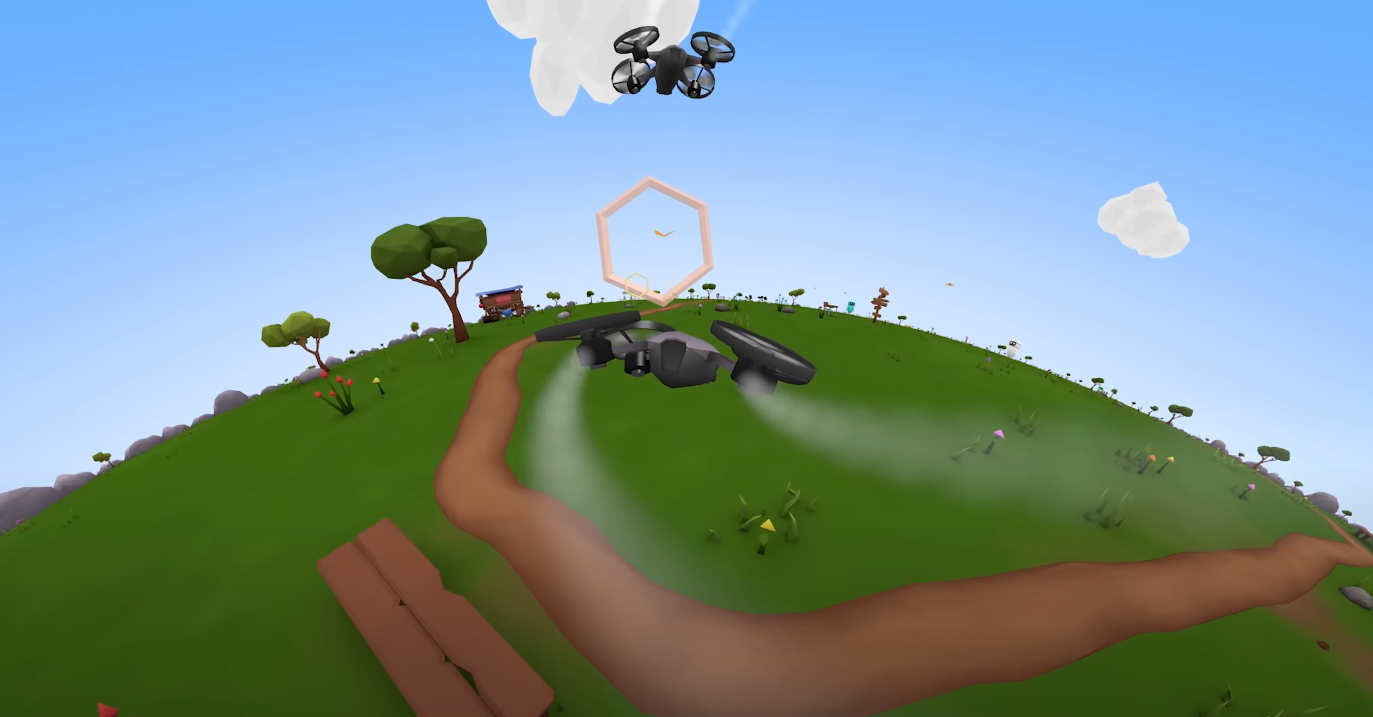
\includegraphics[width=\textwidth]{chapters/results/sections/non_euclidean/resources/hyperbolica-hyperbolic.png}
        \caption[]%
        {{\small \textit{Hyperbolica \cite{Hyperbolica-Hyperbolic}}}}
        \label{fig:hyperbolic-space-games-hyperbolica}
    \end{subfigure}
    \caption[]
    {\small Hyperbolic space}
    \label{fig:hyperbolic-space-games}
\end{figure*}

As mentioned in \autoref{subsubsec:practical-considerations-hyperbolic-space} in our approach the camera's position (as passed to the view matrix) is fixed.
Changing the point where it is located allows us to change the curvature of the terrain.
\autoref{fig:hyperbolic-space-curvatures} shows the scene in hyperbolic space where the camera is positioned close to the origin (cf. \autoref{fig:hyperbolic-space-small-curvature}) resulting in small curvature as compared to the scene when the camera is moved farther from the origin (cf. \autoref{fig:hyperbolic-space-big-curvature}).
\begin{figure*}[h]
    \centering
    \begin{subfigure}[b]{0.475\textwidth}
        \centering
        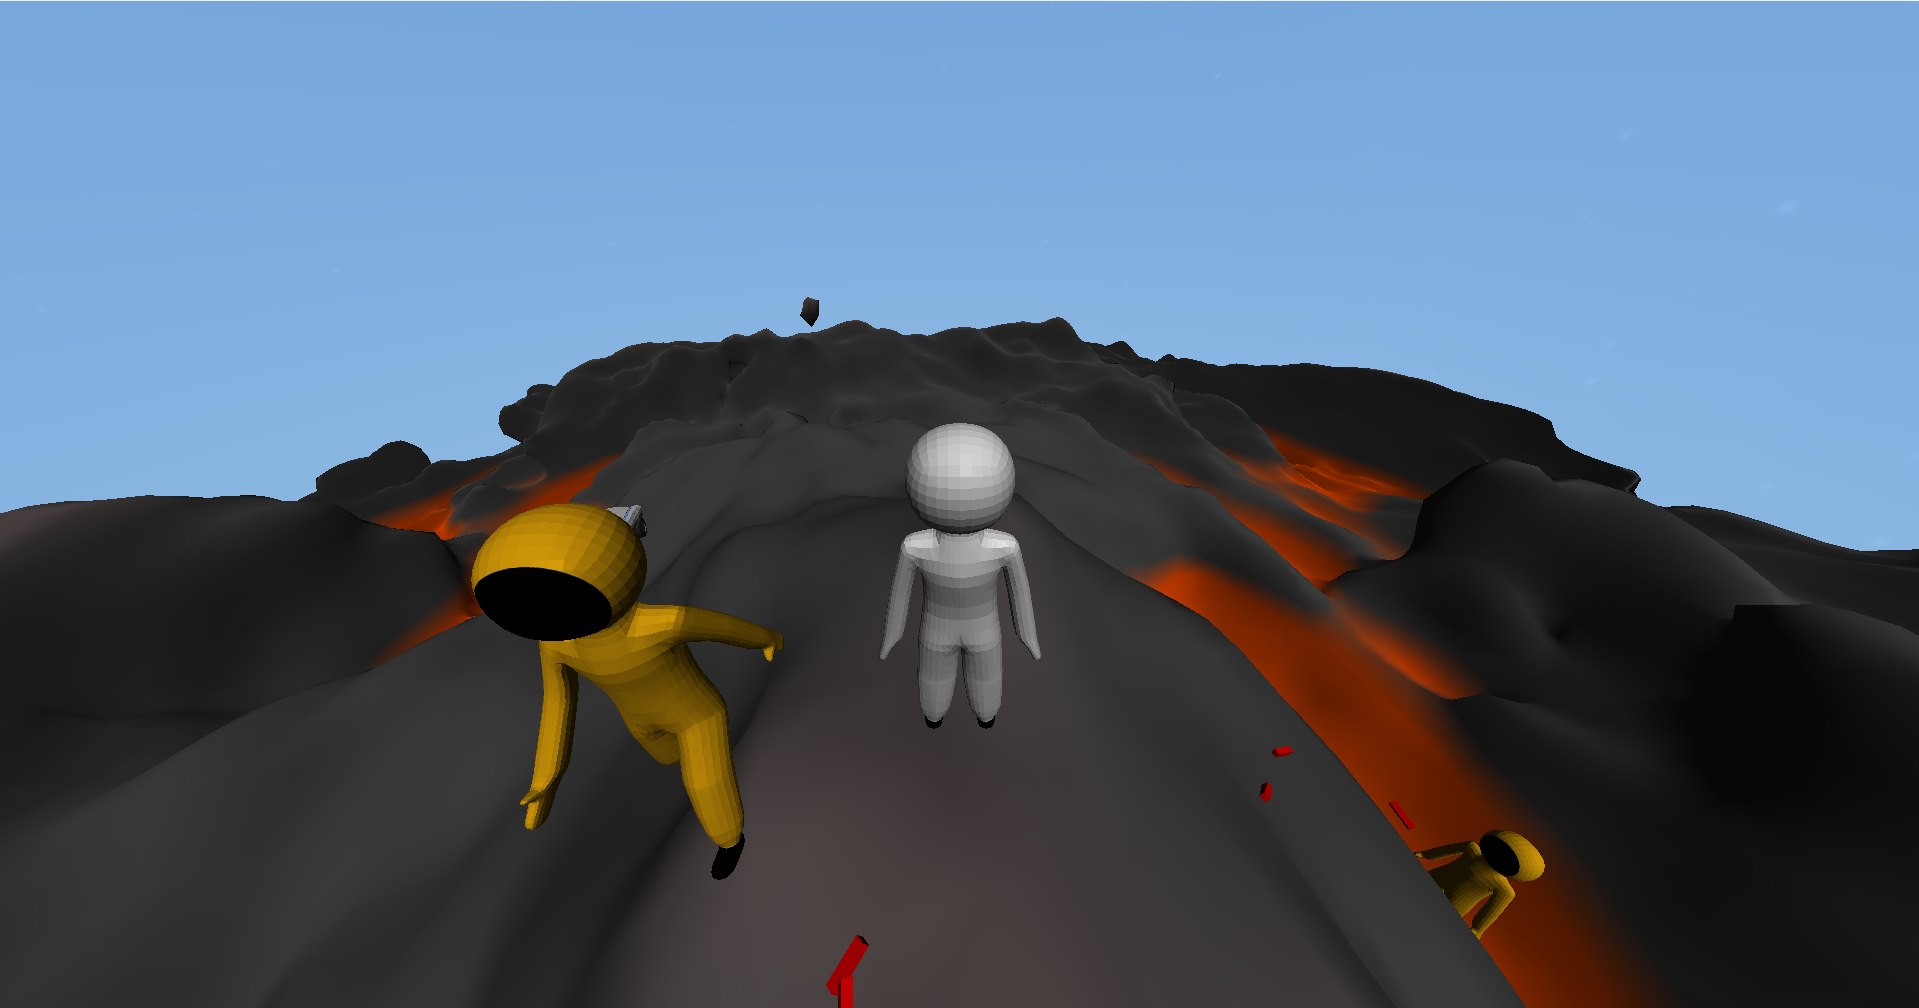
\includegraphics[width=\textwidth]{chapters/results/sections/non_euclidean/resources/hyperbolic-small-curvature.png}
        \caption[]%
        {{\small Camera close to the origin}}
        \label{fig:hyperbolic-space-small-curvature}
    \end{subfigure}
    \hfill
    \begin{subfigure}[b]{0.475\textwidth}
        \centering
        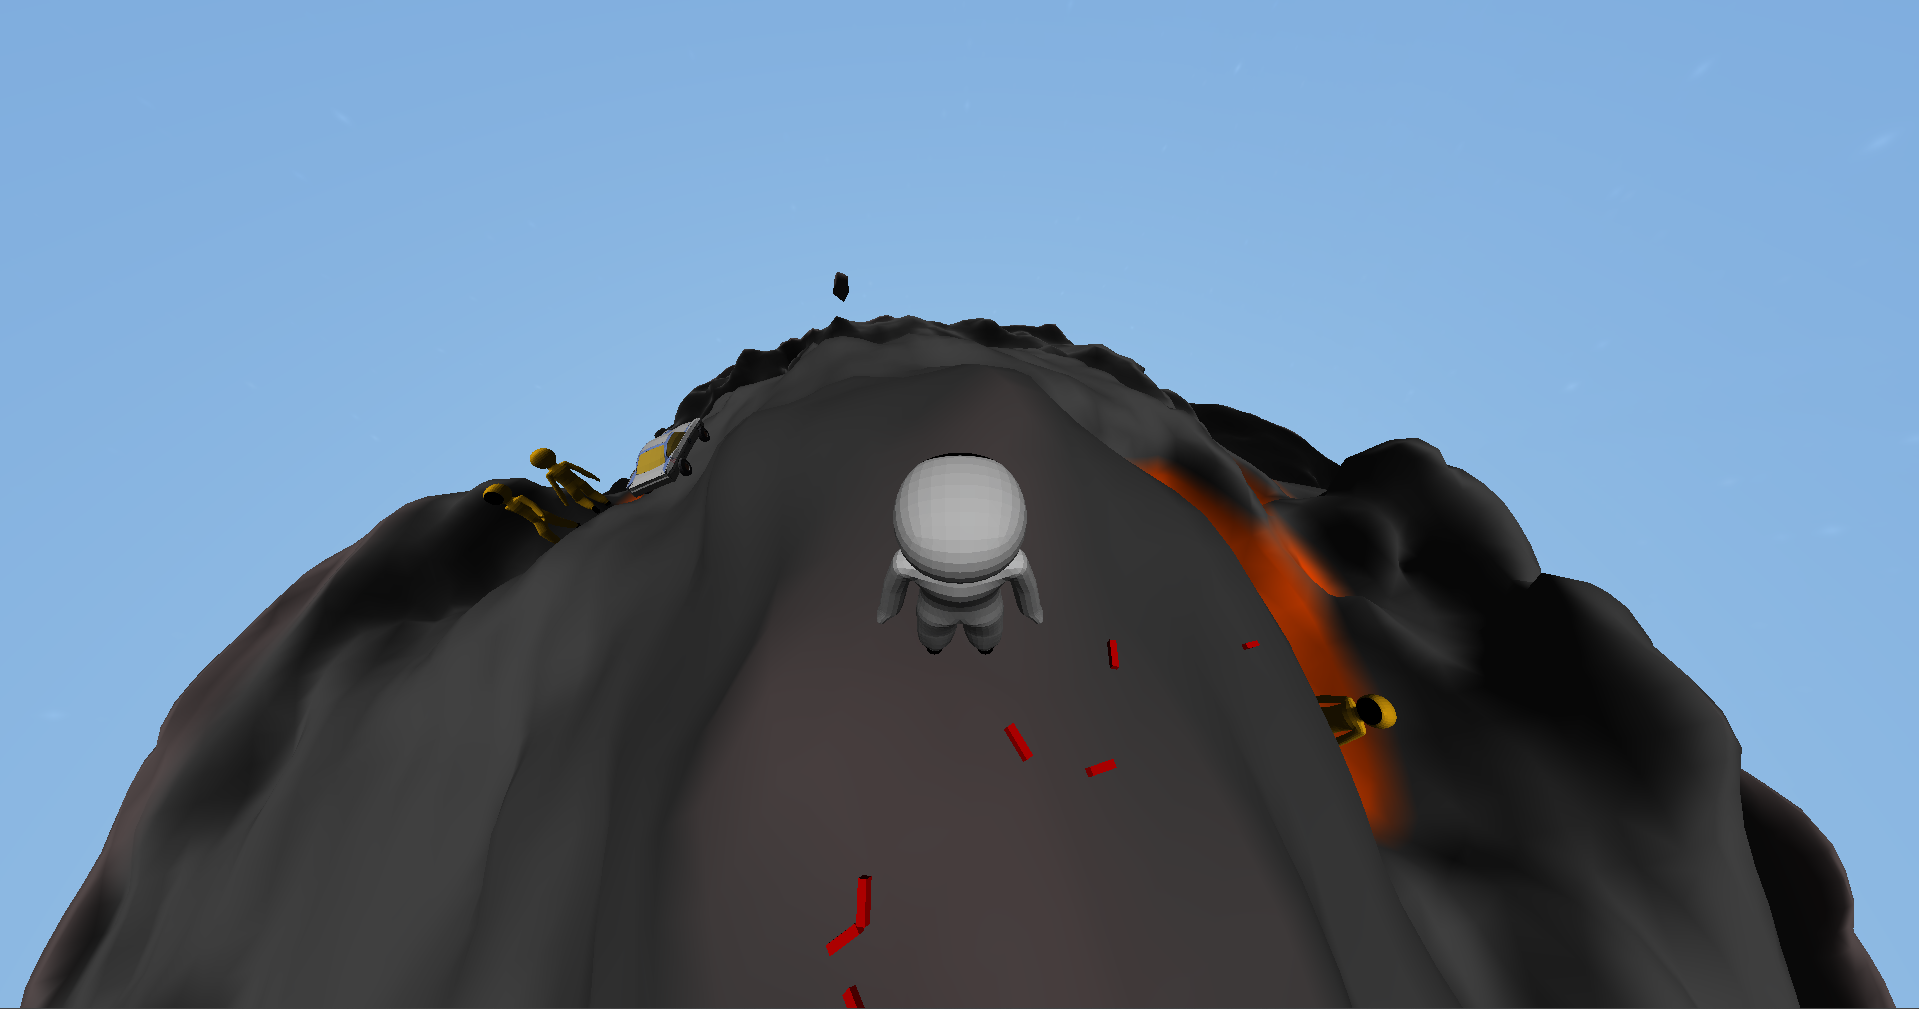
\includegraphics[width=\textwidth]{chapters/results/sections/non_euclidean/resources/hyperbolic-large-curvature.png}
        \caption[]%
        {{\small Camera far from the origin}}
        \label{fig:hyperbolic-space-big-curvature}
    \end{subfigure}
    \caption[]
    {\small Hyperbolic space, different curvatures due to camera's position}
    \label{fig:hyperbolic-space-curvatures}
\end{figure*}

\question{Do we have to mention that our non-Euclidean spaces are "fake" in the sense that you don't have 5-sided right pentagons.}